%===================================================================================================
\subsection{Risk Heterogeneity Among FSW}\label{model.par.fsw}
HIV transmission models which include FSW rarely sub-stratify this population, such as to reflect
differential HIV risk or distinct typologies of sex work \cite{Blanchard2008,Scorgie2012};
yet such heterogeneities likely influence transmission dynamics.
Among the studies identified in Chapter~\ref{sr},
only three sub-stratified FSW by risk-related factors:
\citet{Cremin2017} defined three levels of risk via regression analysis,
\citet{Low2015} distinguished between occasional and full-time FSW, while
\citet{Shannon2015} sub-stratified FSW by
work environment, violence exposure, and context-specific structural factors.
Seven other studies, reflecting two unique models \cite{Johnson2012,Maheu-Giroux2017},
employed age stratification of all activity groups, including FSW;
these models had several risk-related parameters which varied by age.
\par
The model structure here (Figure~\ref{fig:model.risk})
was designed to capture \emph{within}-FSW risk heterogeneity.
The objective of the following analysis was therefore to parameterize
lower \vs higher risk FSW.
I sought to define these groups based on biobehavioural and/or contextual factors
which are demonstrably associated with HIV risk,
and which can be mechanistically incorporated into a transmission model ---
\ie through the force of infection equation.
Later, the parameterization of these groups was validated through model fitting
to relative differences in HIV prevalence \sref{model.cal.targ.prev}.
\par
Many cross-sectional studies of HIV among FSW quantify
the association of risk factors with HIV serostatus
\cite{Aklilu2001,Dunkle2005,Scorgie2012,Jonas2020}.
However, serostatus reflects cumulative risk exposure,
whereas sexual risk behaviour is dynamic \cite{Watts2010,vanWees2020},
as is use of prevention resources \cite{Roberts2020}.
For example, while HIV prevalence often increases with age,
HIV incidence among women can peak shortly after sexual debut \cite{Dellar2015}.
Thus, risk factors associated with HIV serostatus are not necessarily
mechanistically related to HIV acquisition.
Indeed, FSW may reduce risk behaviours in response to seroconversion \cite{McClelland2006}.
Cohort studies that measure incidence
can help identify risk factors for HIV acquisition \cite{McKinnon2015,Nouaman2022},
but large sample sizes are often required to accurately estimate overall incidence rate,
let alone risk factors \cite{Priddy2011}.
%---------------------------------------------------------------------------------------------------
\subsubsection{FSW Survey Data}\label{model.par.fsw.data}
Three surveys, in
2011 \cite{Baral2014} (N = 325),
2014 \cite{EswKP2014} (N = 781), and
2021 \cite{EswIBBS2022} (N = 676)
provide HIV and biobehavioural data on FSW in Eswatini.
The 2011 survey employed respondent driven sampling (RDS, details in \cite{Yam2013}),
as did the 2021 survey.
The 2014 survey employed venue-based snowball sampling, based on the
Priorities for Local AIDS Control Efforts (PLACE) methodology,
which aims to identify areas of higher incidence \cite{Weir2005}.
I analyzed the individual-level data from 2011 and 2014 (data from 2021 not yet available)
to explore the potential association of biobehavioural factors with HIV risk,
so that such factors could then be used to distinguish between
lower risk \vs higher risk FSW.
%---------------------------------------------------------------------------------------------------
\subsubsection{HIV Status}\label{model.par.fsw.hiv}
Only the 2011 and 2021 studies included serologic testing for HIV.
Among those tested in 2011 (N = 317, 98\%), 70\% were \hivp,
yielding RDS-adjusted prevalence estimate of 61\% (CI: 51--71\%) \cite{Baral2014}.
Among serologically \hivn, 11\% self-reported \hivp status (false positive), and
among serologically \hivp, 26\% self-reported \hivn status (false negative or undiagnosed).
Overall, self-reported HIV status underestimated HIV prevalence in 2011
by a factor of approximately 0.78 (55~vs~70\%).
Unadjusted HIV prevalence in 2021 was 58.8\%,
with 88\% (363/411) reporting previous awareness of \hivp status.
\par
In 2014, self-reported HIV prevalence was 38\% among respondents who reported (85\%).
This 38\% is surprisingly low considering that
the PLACE methodology explicitly aimed to sample venues
with higher HIV incidence \cite{Weir2005}, and 2014 \vs 2011 respondents
were older (median 27 \vs 25 years), % 2021 median: 28
had been selling sex longer (median 5 \vs 4 years), % 2021: 6
and tested more frequently (87 \vs 75\% tested at least once in the past year, % 2021: 75
82 \vs 63\% among self-reported \hivn).
Perhaps the differences are attributable to the sampling methodology.
Among respondents who self-reported \hivp status,
the 2014 survey also asked for age of HIV diagnosis (6\% missing).
Age of HIV diagnosis supports crude time-to-event analysis (next section),
which can account for confounding by age and censoring,
as compared to logistic regression on HIV status,
keeping in mind the limitations of self-reported HIV status.
%---------------------------------------------------------------------------------------------------
\subsubsection{Risk Factors}\label{model.par.fsw.fac}
Next, I explored the potential association of risk factors with HIV
via the following three models:%
\footnote{Logistic regression models were implemented using \texttt{lrm} from:
  \hreftt{cran.r-project.org/package=rms}.\\
Cox proportional hazards models were implemented using \texttt{coxaalen} from:
  \hreftt{cran.r-project.org/package=coxinterval}.}
\begin{enumerate}
  \item Logistic regression on serologic HIV status (2011 data)
  \item Logistic regression on self-reported HIV status (2014 data)
  \item Cox proportional hazards for interval-censored time to HIV infection,
    with interval from self-reported sex work debut 
    to either self-reported time of HIV diagnosis or survey date (2014 data);
    Figure~\ref{fig:fsw.tte.interval} illustrates
    the four potential censoring cases in this framework.
\end{enumerate}
An important limitation to all models is that
risk factors reported by FSW at the time of survey
are assumed to be fixed characteristics of the respondents,
rather than dynamic characteristics that vary over time.
Additionally, respondents with any missing variables for each individual model
were excluded from that model. % TODO: (%)
\begin{figure}
  \centering
  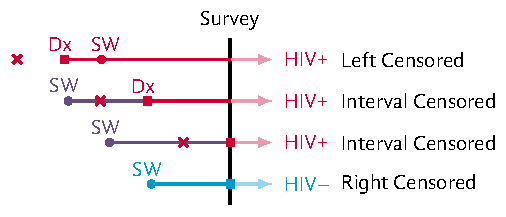
\includegraphics[scale=1]{diag.tte}
  \caption{Illustration of time-to-event analysis framework
    for cross-sectional FSW survey data}
  \label{fig:fsw.tte.interval}
  \floatfoot{
    $\bm{\times}$: HIV infection;
    SW: time of sex work debut;
    Dx: time of HIV diagnosis.}
\end{figure}
\par
Risk factors were selected based on
prior knowledge of plausible mechanistic influence on HIV incidence and/or prevalence.
The risk factors explored are summarized in Table~\ref{tab:fsw.stats},
including univariate and multivariable association under each model.
Variable selection for multivariable models
was performed using backward selection as described by \citet{Lawless1978},
using a $p \le 0.1$ (per variable) threshold for stepwise variable retention.
Estimated conditional effects of
variables retained in the multivariable logistic regression models
are illustrated in Figure~\ref{fig:fsw.lr}.
\begin{table}
  \centering
  \caption{Risk factors explored for association with \hivp status among FSW in Eswatini}
  \label{tab:fsw.stats}
  \centerline{%
\small%
\begin{tabular}{lcccccccccccc}
  \toprule
  & \multicolumn{4}{c}{2011 LR}
  & \multicolumn{4}{c}{2014 LR}
  & \multicolumn{4}{c}{2014 CPH} \\
  \cmidrule(rl){2-5}\cmidrule(rl){6-9}\cmidrule(rl){10-13}
  & \multicolumn{2}{c}{Univar} & \multicolumn{2}{c}{Multivar}
  & \multicolumn{2}{c}{Univar} & \multicolumn{2}{c}{Multivar}
  & \multicolumn{2}{c}{Univar} & \multicolumn{2}{c}{Multivar} \\
  \cmidrule(rl){2-3}\cmidrule(rl){4-5}\cmidrule(rl){6-7}\cmidrule(rl){8-9}\cmidrule(rl){10-11}\cmidrule(rl){12-13}
  Factor                          &  OR  &   p   &  OR  &   p    &  OR  &   p    &  OR  &   p    &  HR  &   p    &  HR  &   p    \\
  \midrule                        % 2011 LR uni  % 2011 LR multi % 2014 LR uni   % 2014 LR multi % 2014 CPH uni  % 2014 CPH multi
  Age\tn{a}                       & 1.11 & \vsig & ---  &  ---   & 1.14 & \vsig  & 1.15 & \vsig  & 1.09 & \vsig  & 1.09 & \vsig  \\
  Years selling sex\tn{a}         & 1.13 & \vsig & 1.13 & \vsig  & 1.12 & \vsig  & ---  &  ---   & 1.08 & \vsig  & ---  &  ---   \\
  Monthly sex work income\tn{b}   & 0.98 & 0.155 & ---  &  ---   & 0.98 & 0.097  & 0.97 & 0.084  & 0.98 & 0.019\s& 0.97 & 0.001\s\\[1ex]
  Non-paying partners\tn{c}       & 0.88 & 0.307 & ---  &  ---   & 1.07 & 0.233  & ---  &  ---   & 1.05 & 0.312  & ---  &  ---   \\
  Monthly new clients\tn{c}       & 1.01 & 0.412 & ---  &  ---   & 1.05 & \vsig  & 1.07 & \vsig  & 1.04 & \vsig  & 1.04 & \vsig  \\
  Monthly regular clients\tn{c}   & 1.01 & 0.351 & ---  &  ---   & 1.03 & 0.002  & ---  &  ---   & 1.02 & \vsig  & 1.02 & 0.034\s\\[1ex]
  Non-paying condom use\tn{d}     & 0.90 & 0.703 & ---  &  ---   & 0.90 & 0.673  & ---  &  ---   & 0.92 & 0.677  & ---  &  ---   \\
  New client condom use\tn{d}     & 0.60 & 0.100 & ---  &  ---   & 0.48 & 0.006\s& 1.25 & 0.599  & 0.56 & 0.004\s& ---  &  ---   \\
  Regular client condom use\tn{d} & 0.58 & 0.110 & ---  &  ---   & 0.39 & \vsig  & 0.35 & 0.004\s& 0.49 & \vsig  & 0.50 & \vsig  \\[1ex]
  Any anal sex past month         & 0.97 & 0.896 & ---  &  ---   & 1.89 & 0.015\s& ---  &  ---   & 1.57 & 0.015\s& 1.27 & 0.260  \\
  Any STI symptoms past year      & 2.29 & \vsig & 2.41 & \vsig  & 2.75 & \vsig  & 2.80 & \vsig  & 2.17 & \vsig  & 2.05 & \vsig  \\
  \bottomrule
\end{tabular}}
% TODO: HIV status?
\floatfoot{\raggedright
  \tnt[a]{OR per year};
  \tnt[b]{OR per Swati lilangeni per month};
  \tnt[c]{OR per partner};
  \tnt[d]{2011: always vs not always, 2014: at last sex}.
  --- indicates variable was not selected in the multivariate model.
  LR: logistic regression on HIV$+/-$ status;
  CPH: Cox proportional hazards on time to self-reported HIV seroconversion.
  OR: odds ratio; HR: hazard ratio; p: p-value.
  2011 data based on serologic HIV test;
  2014 data based on self-reported HIV status, age of sex work debut, and age of HIV diagnosis.
}
\end{table}
\begin{figure}[h]
  \subcaptionoverlap
  \foreach \year/\var/\nvar in {2011/f/1,2011/c/2,2014/f/3,2014/c/3}{
  \begin{subfigure}{\nvar\linewidth/5+\linewidth/5}
    \includegraphics[scale=.7]{fsw.\year.lr.hiv.\var}
    \caption{\raggedright}
    \label{fig:fsw.lr.\year.\var}
  \end{subfigure}}
  \caption{Predicted conditional effects (probability)
    of variables in multivariable logistic regression models for HIV status}
  \label{fig:fsw.lr}
  \floatfoot{\fffsw{fig:fsw.lr}
    conditional probabilities shown for fixed covariates at arbitrary values.}
\end{figure}
\par
Following variable selection, each multivariable model was used to predict
the total \hivp status odds ratio (logistic) or HIV incidence hazard ratio (Cox)
for each respondent in the respective survey ---
\ie $e^{X_i\,\beta}$ for respondent $i$ ---
representing an overall ``risk score'' under each model.
Respondents were then stratified into the top 20\% and bottom 80\% by these risk scores.
The values of each variable were compared between these two strata
using a test for the ratio of the means \cite{Tamhane2004} to support model parameterization;
these ratios are summarized in Table~\ref{tab:fsw.ratios},
and the distributions of variable values across the two strata
are illustrated in Figure~\ref{fig:fsw.f}.
\begin{table}
  \centering
  \caption{Ratios of HIV risk factor variables among higher \vs lower risk FSW in Eswatini}
  \label{tab:fsw.ratios}
  \centerline{\footnotesize%
\begin{tabular}{lcccccc}
  \toprule
  & \multicolumn{2}{c}{2011 LR}
  & \multicolumn{2}{c}{2014 LR}
  & \multicolumn{2}{c}{2014 CPH} \\
  \cmidrule(rl){2-3}\cmidrule(rl){4-5}\cmidrule(rl){6-7}
  Factor                            &  High / Low   &   Ratio (95\% CI)   &  High / Low   &   Ratio (95\% CI)   &   High / Low   &   Ratio (95\% CI)   \\
  \midrule
  Age                               & 31.8  / 24.7  & 1.29 (1.22, 1.36)\s & 32.6  / 26.2  & 1.24 (1.20, 1.28)\s &  33.5  / 26.6  & 1.26 (1.21, 1.31)\s \\
  Years selling sex                 & 11.3  /  4.03 & 2.81 (2.41, 3.25)\s & 10.0  /  5.47 & 1.83 (1.64, 2.03)\s &  10.2  /  5.83 & 1.75 (1.54, 1.98)\s \\
  Monthly sex work income\tn{a}     & 15.1  / 15.2  & 1.00 (0.86, 1.15)   &  6.77 /  7.06 & 0.96 (0.82, 1.11)   &   6.32 /  7.28 & 0.87 (0.73, 1.02)   \\[1ex]
  Non-paying partners               &  1.42 /  1.43 & 0.99 (0.81, 1.19)   &  1.56 /  1.11 & 1.40 (1.11, 1.72)\s &   1.53 /  1.19 & 1.29 (0.98, 1.62)   \\
  Monthly new clients               &  5.50 /  6.98 & 0.79 (0.49, 1.15)   &  8.39 /  4.15 & 2.02 (1.63, 2.44)\s &   8.36 /  4.41 & 1.90 (1.43, 2.39)\s \\
  Monthly regular clients           &  9.35 /  9.05 & 1.03 (0.69, 1.42)   & 11.1  /  8.25 & 1.35 (1.13, 1.57)\s &  12.4  /  8.61 & 1.44 (1.18, 1.71)\s \\[1ex]
  Non-paying condom use\tn{bc}      &  0.26 /  0.35 & 0.73 (0.40, 1.11)   &  0.77 /  0.81 & 0.95 (0.84, 1.06)   &   0.76 /  0.81 & 0.95 (0.81, 1.08)   \\
  New client condom use\tn{bc}      &  0.68 /  0.76 & 0.89 (0.73, 1.06)   &  0.79 /  0.91 & 0.86 (0.79, 0.94)\s &   0.74 /  0.94 & 0.79 (0.69, 0.88)\s \\
  Regular client condom use\tn{bc}  &  0.38 /  0.46 & 0.83 (0.45, 1.28)   &  0.67 /  0.91 & 0.74 (0.65, 0.82)\s &   0.60 /  0.92 & 0.65 (0.55, 0.75)\s \\[1ex]
  Any anal sex past month           &  0.59 /  0.41 & 1.41 (1.06, 1.84)\s &  0.17 /  0.07 & 2.43 (1.47, 3.85)\s &   0.23 /  0.07 & 3.24 (1.95, 5.34)\s \\
  Any STI symptoms past year\tn{c}  &  0.79 /  0.43 & 1.86 (1.54, 2.25)\s &  0.59 /  0.15 & 3.94 (3.15, 5.03)\s &   0.61 /  0.17 & 3.67 (2.87, 4.79)\s \\[1ex]
  HIV prevalence\tn{d}              &  0.94 /  0.64 & 1.46 (1.30, 1.63)\s &  0.66 /  0.29 & 2.29 (1.92, 2.75)\s &   0.71 /  0.31 & 2.32 (1.94, 2.80)\s \\
  \bottomrule
\end{tabular}}
\floatfoot{\raggedright
  High / Low: mean variable value among higher / lower risk groups, as defined by
  the top 20\% / bottom 80\% in multivariable model-predicted risk score:
  odds ratio from logistic regression (LR);
  hazards ratio from Cox proportional hazards (CPH).
  \tnt[a]{Swati lilangeni per month};
  \tnt[b]{2011: always \vs not always, 2014: did use condom at last sex};
  \tnt[c]{proportion of respondents};
  \tnt[d]{2011: serologic HIV status; 2014: self-reported HIV status};
  \tnt[*]{statistically significant, $p < 0.05$}.
}
\end{table}
